%Pieces of code to be copied in report
%Please change all text between ** 
%Abbreviated name is the name in a few words (So we can reference to it easily)

%% ################### SI Stuff ############
\SI{}{}
use \newton and \gram etc.
and \kilo and \milli etc.
and \per for the division line

%% ################### Referencing & citing ###################
%Refrencing
\autoref{<label>}

%Citiation
\cite[<note>,<note2>]{<source>}


%% ################### Chapters & Sections ###################
%Code to add chapter
\chapter{*Name of chapter*}
\label{Ch_*Abbreviated chapter name*}

%Code for section
\section{*Name of section*}
\label{Sec_*Abbreviated chapter name*_*Abbreviated section name*}

%Code subsection
\subsection{*Name of subsection*}
\label{SubSec_*Abbreviated chapter name*_*Abbreviated section name*_Abbreviated subsection name*}

%% ################### Tables & Lists ###################
%Code for manual table creation (there is also a excel add-on to export tables to latex, a online version can be found here: https://www.tablesgenerator.com/)
\begin{table}[H]
\centering
\caption{*caption*}
    \begin{tabular}{l p{7cm} p{7cm}}
        \rowcolor{Blue}
           &  &  \\
        1) &  &  \\
        2) &  &  \\
        n) &  &  \\
    \end{tabular}
    \label{table:*name*}
\end{table}

%Code for table structure
|,c,l,r,p{<n>cm} %line between columns,centered column, left aligned column, right aligned column, column of specified width
\rowcolor{},\hline,\midrule,\toprule,\bottomrule %Different types of lines and markings. Put these between the rows.

%Code for bullet points and lists
\begin{itemize}
  \item One entry in the list
  \item Another entry in the list
\end{itemize}


%% ################### Equations ###################
%Equations (equations don't have captions and must be mentioned (using \autoref) in the text)
\begin{equation}
    \label{Eq_*Abbreviated Capter*_*Calculated Variable Name*}
    *Calculated variable*=*Multi variable part*
\end{equation}

%Useful code for in equations, please ask if anything is unclear
%   \*symbol*               for any symbol not on the keyboard
%   _{*Subscript*}          for subscript
%   ^{*Super script*}       for superscript
%   * multiplication        for multiplication
%   \frac{*top*}{*bottom*}  for all fractions

%Code for bullet points and lists


\begin{itemize}
  \item One entry in the list
  \item Another entry in the list
\end{itemize}






%% ################### Figures ###################
%FIGURES (Note: all images and illustrations should be placed in the figures folder regardless of where they are in the report)

%Standard figure
\begin{figure}[h!]
    \centering
    \includegraphics[width=0.5\textwidth]{figures/*filename.fileextension*}
    \caption{*Caption of figure*}
    \label{Fig_*Abbreviated Capter*_*Abbreviated caption*}
\end{figure}


%Code for figures with sub-figures (copy the sub-figure section for each sub-figure)
\begin{figure}[h!]
\begin{subfigure}[b]{0.5\textwidth}
    \centering
    \includegraphics[width=1\textwidth]{figures/*filename.fileextension*}
    \caption{*Figure sub-caption*}
    \label{SubFig_*Abbreviated Capter*_*Abbreviated sub-caption*}
\end{subfigure}
\caption{*Caption for all figures*}
\label{Fig_*Abbreviated Capter*_*Abbreviated caption*}
\end{figure}

%Wrapped figure (figure next to text (please ask someone for help when using for the first time, this one has the tendency to act a little weird))
\begin{wrapfigure}{r}{0.5\textwidth}
    \centering
    \includegraphics[width=0.5\textwidth]{figures/*filename.fileextension*}
    \caption{*Caption of figure*}
    \label{Fig_*Abbreviated Capter*_*Abbreviated caption*}
\end{wrapfigure}


%% ################### Plots ###################
%For those who don't want Excel screenshots in there report, there is LaTeX plots. Those plots support a multitude of plot types and inputs. Here under you can find an example of a basic line graph. As the pgfplots package is quite extensive I won't write all the possible configurations here. I do present to you, the pgfplots manual: http://pgfplots.net/media/pgfplots/pgfplots.pdf (it includes step by step tutorials)

\begin{center}
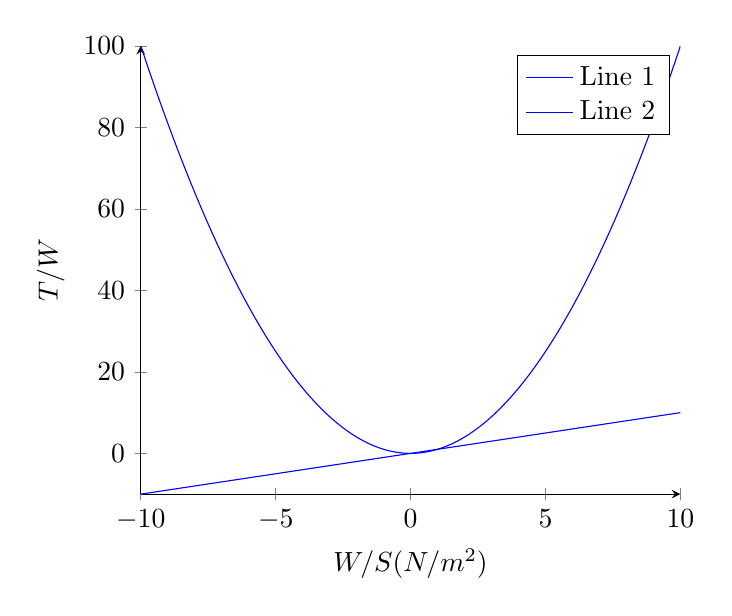
\begin{tikzpicture}
\begin{axis}[
    axis lines = left,
    xlabel = $W/S (N/m^2)$,
    ylabel = {$T/W$},
]
%Line 1 is defined
\addplot [
    domain=-10:10, 
    samples=100, 
    color=blue,
]
{x^2}; %#### Line Eq. here
\label{Plt:Line1}
\addlegendentry{Line 1}
%Line 2 is defined
\addplot [
    domain=-10:10, 
    samples=100, 
    color=blue,
]
{x};
\label{Plt:Line2}
\addlegendentry{Line 2}



%Graph as a result of a .dat file
\end{axis}
\end{tikzpicture}
\end{center}

\begin{center}
\begin{tikzpicture}
\begin{axis}[
    title = Aircraft comparison,
    axis lines = left,
    xlabel = $label$,
    ylabel = {label},
]
\addplot [] table {test.dat};

\end{axis}
\end{tikzpicture}
\end{center}




